\documentclass[12pt,a4paper]{article}

% ------------------------------------------------
% Paquetes
% ------------------------------------------------
\usepackage[utf8]{inputenc}
\usepackage[T1]{fontenc}
\usepackage[spanish, es-nodecimaldot]{babel}
\usepackage{geometry}
\usepackage{graphicx}
\usepackage{float}
\usepackage{xcolor}
\usepackage{listings}
\usepackage{hyperref}
\usepackage{fancyhdr}
\usepackage{titlesec}

% ------------------------------------------------
% Configuración de página
% ------------------------------------------------
\geometry{
    top=2.5cm,
    bottom=2.5cm,
    left=2.5cm,
    right=2.5cm
}

% ------------------------------------------------
% Configuración de listings
% ------------------------------------------------
\definecolor{codegray}{gray}{0.95}

\lstset{
    backgroundcolor=\color{codegray},
    basicstyle=\ttfamily\small,
    breaklines=true,
    frame=single,
    columns=fullflexible,
    keepspaces=true
}

% ------------------------------------------------
% Encabezado y pie de página
% ------------------------------------------------
\pagestyle{fancy}
\fancyhf{}
\lhead{Interacción de redes}
\rhead{Práctica 5}
\cfoot{\thepage}

% ------------------------------------------------
% Configuración de títulos
% ------------------------------------------------
\titleformat{\section}
{\large\bfseries}
{\thesection.}
{0.5em}
{}

% ------------------------------------------------
% Hipervínculos
% ------------------------------------------------
\hypersetup{
    colorlinks=true,
    linkcolor=black,
    urlcolor=blue,
    citecolor=black
}

% ------------------------------------------------
% Datos del documento
% ------------------------------------------------
\title{
    Práctica 5: Modificación de ACL estándar\\[0.5em]
    \large Interacción de redes
}

\author{
    Jorge Alberto Suarez Saldana\\
    \small Matrícula: 355992\\
    \small Profesor: Raymundo Antonio González Grimaldo
}

\date{\today}

% ------------------------------------------------
% Documento
% ------------------------------------------------
\begin{document}

\maketitle

\section{Introducción}

En esta práctica se realizó la modificación y configuración de
listas de control de acceso (ACL) estándar en los dispositivos de
red. Se verificó la configuración mediante el comando
\texttt{show access-lists} y se realizaron pruebas de conectividad
en Packet Tracer para comprobar el comportamiento de las reglas
establecidas.

Las ACL permiten controlar el tráfico que puede atravesar una
interfaz de un dispositivo de red mediante reglas que especifican
qué tráfico debe ser permitido o denegado.

\section{Configuración y verificación}

Una vez realizadas las modificaciones correspondientes a las ACL
estándar, se verificó su configuración mediante el comando:

\begin{lstlisting}
show access-lists
\end{lstlisting}

La salida obtenida en el router R1 se muestra a continuación.

\begin{figure}[H]
    \centering
    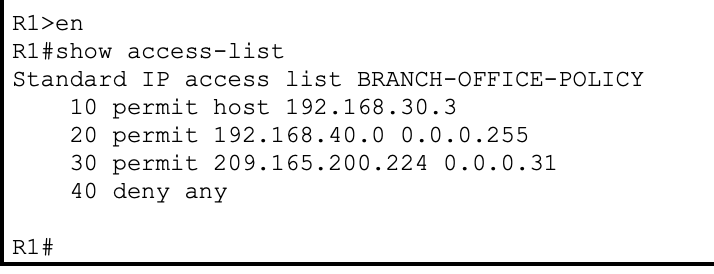
\includegraphics[width=0.95\textwidth]{access-listR1.png}
    \caption{Salida de \texttt{show access-lists} en R1.}
    \label{fig:access-list-r1}
\end{figure}

De manera similar, se verificó la configuración de las listas de
control de acceso en R3.

\begin{figure}[H]
    \centering
    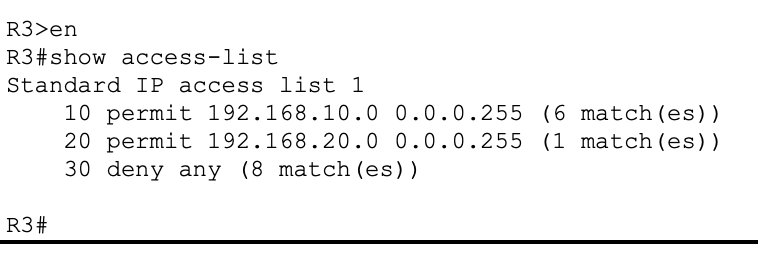
\includegraphics[width=0.95\textwidth]{access-listR3.png}
    \caption{Salida de \texttt{show access-lists} en R3.}
    \label{fig:access-list-r3}
\end{figure}

Las capturas anteriores permiten comprobar que las ACL fueron
creadas con las reglas correspondientes y que se encuentran
configuradas en los dispositivos de acuerdo con los requerimientos
de la práctica.

\section{Resultados}

Para comprobar el funcionamiento de las ACL se realizaron pruebas
de conectividad en Packet Tracer. Así mismo, los resultados obtenidos, verificados por la pestaña Assessment-Items se
muestran en la Figura~\ref{fig:results}.

\begin{figure}[H]
    \centering
    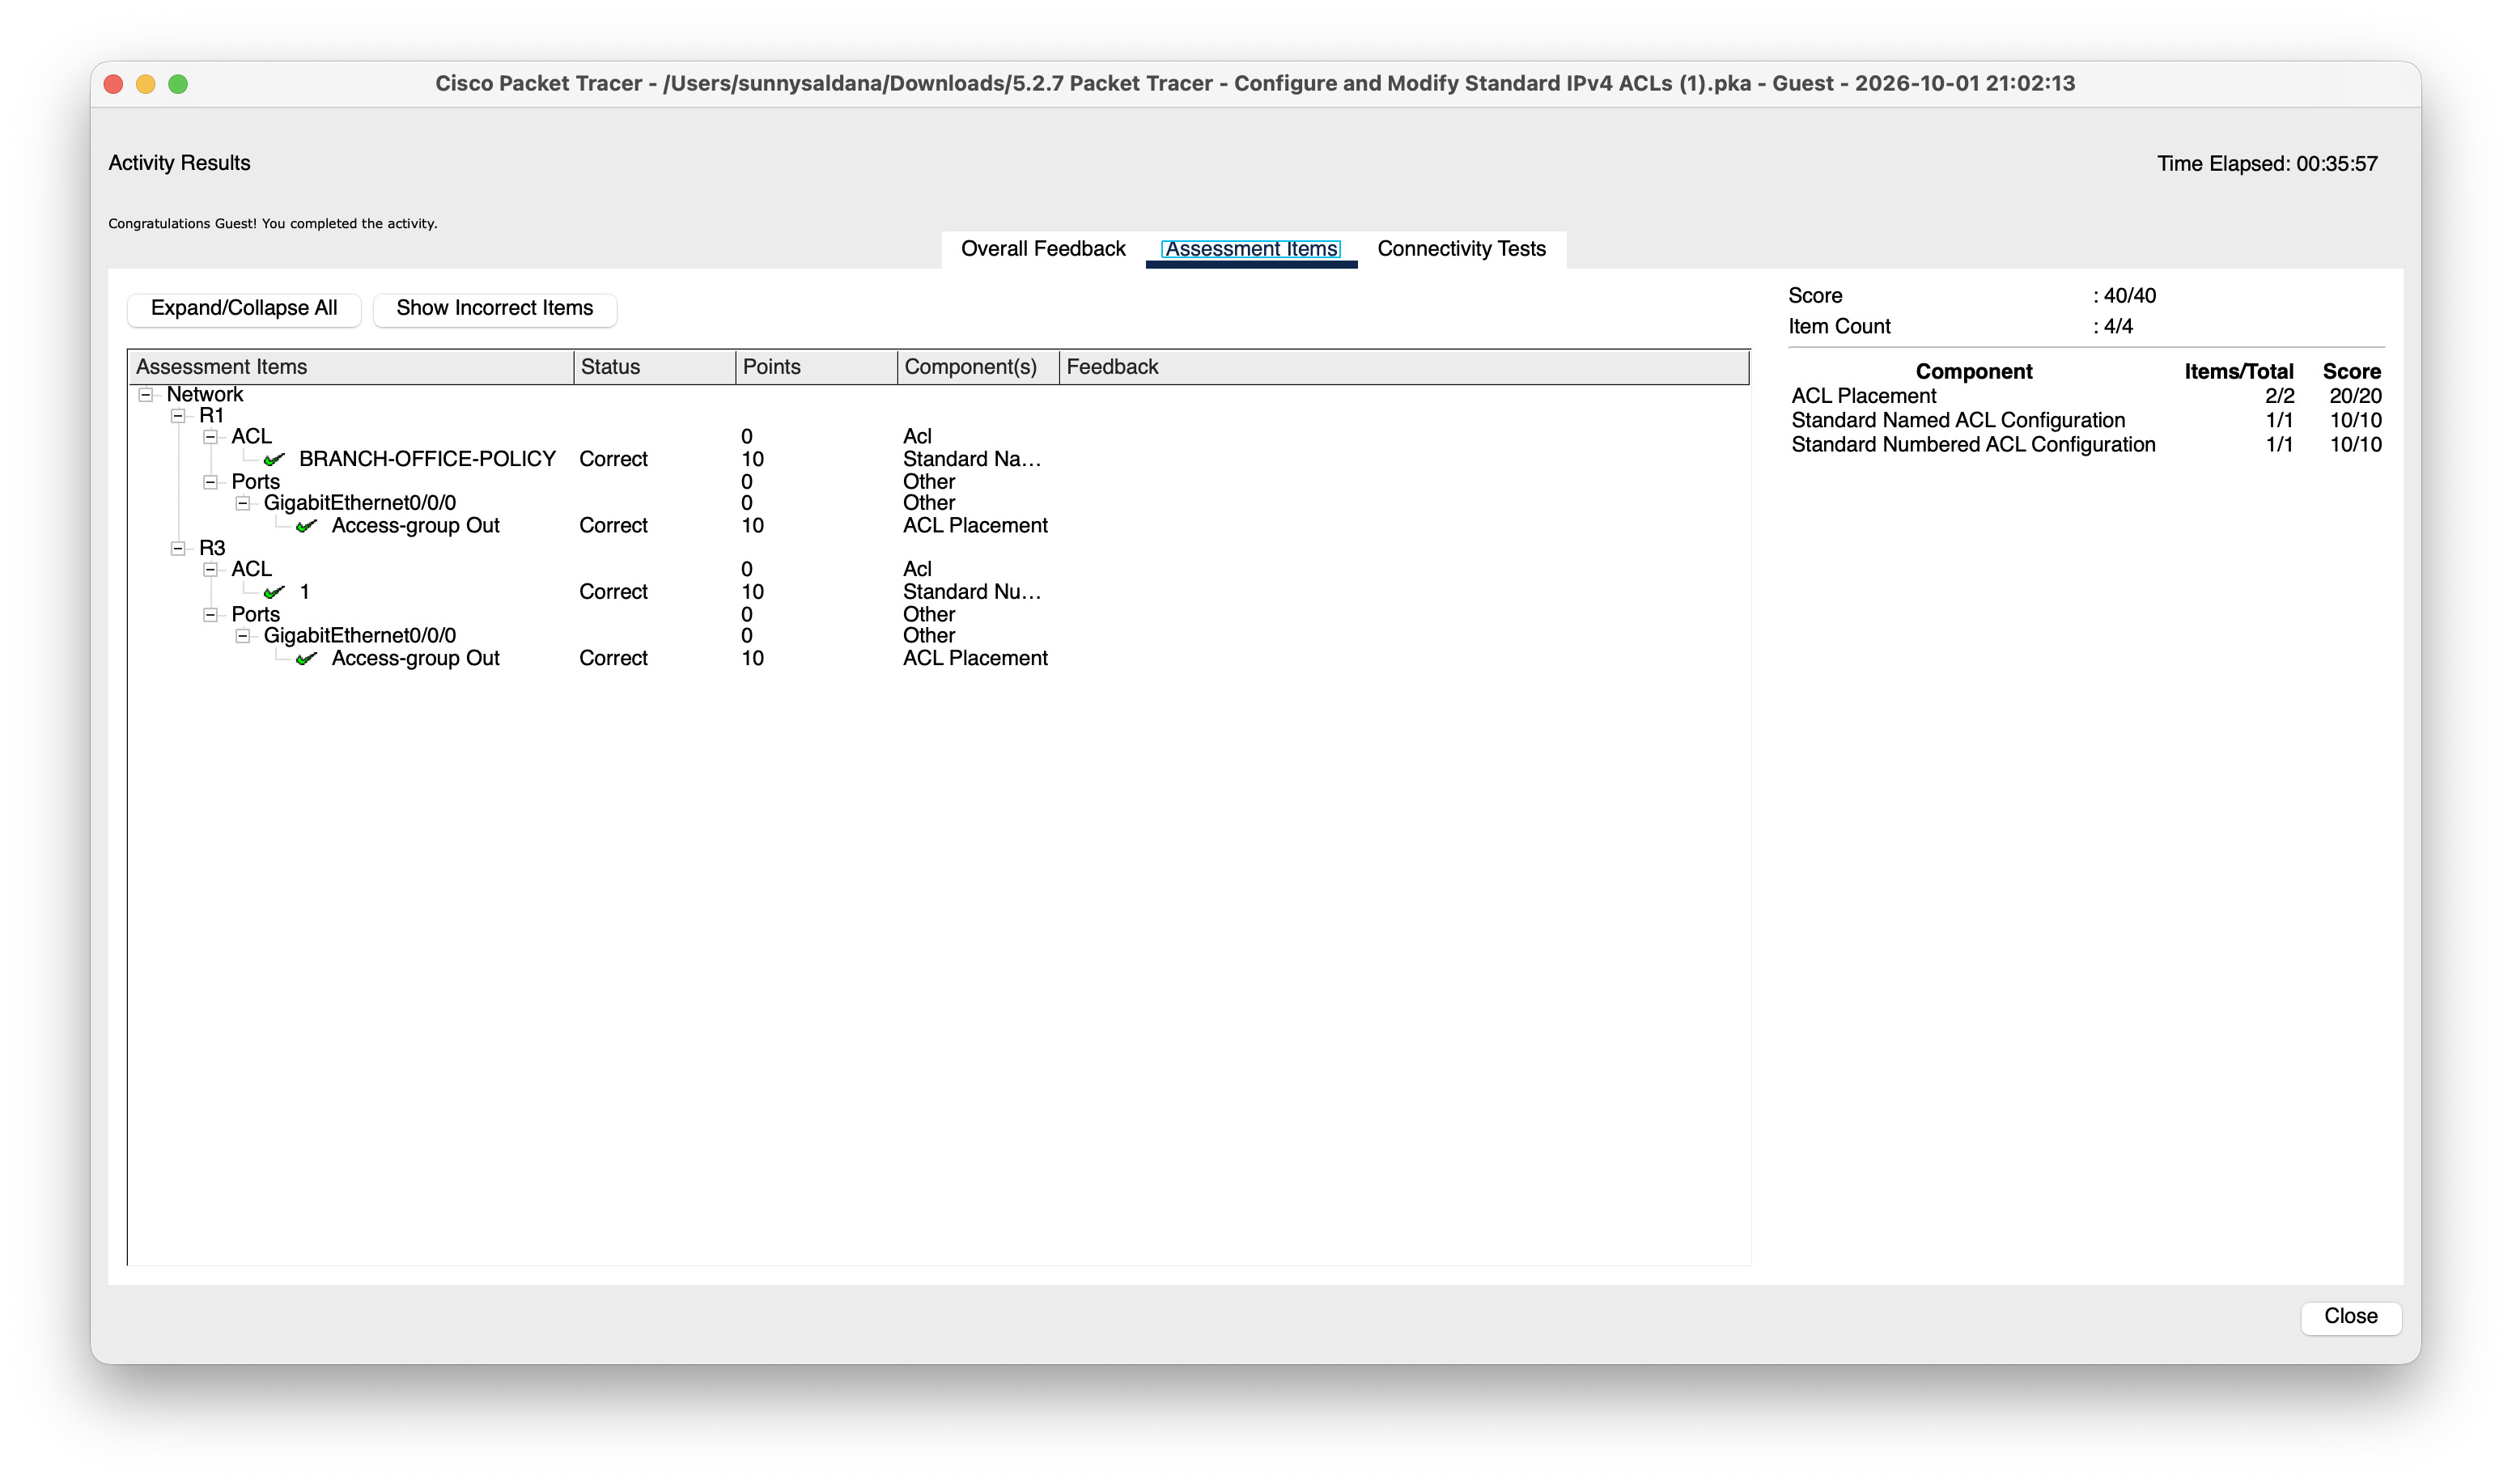
\includegraphics[width=\textwidth]{results.png}
    \caption{Resultados de las pruebas realizadas en Packet Tracer.}
    \label{fig:results}
\end{figure}

A partir de estas pruebas se pudo verificar el comportamiento de las
ACL configuradas, observando qué comunicaciones fueron permitidas
y cuáles fueron bloqueadas de acuerdo con las reglas establecidas.

\section{Preguntas}

\subsection{¿Por qué tendría la necesidad de usar ACL extendidas?}

Las ACL estándar permiten controlar el tráfico principalmente con
base en la \textbf{dirección IP de origen}. Esto resulta suficiente
cuando únicamente se necesita determinar qué redes o dispositivos
pueden enviar tráfico a través de una interfaz.

Sin embargo, existen situaciones en las que se necesita un control
mucho más específico. Las ACL extendidas permiten establecer
condiciones adicionales, como:

\begin{itemize}
    \item Dirección IP de origen.
    \item Dirección IP de destino.
    \item Protocolo utilizado, como TCP, UDP o ICMP.
    \item Puertos de origen y destino.
    \item Determinados tipos de tráfico.
\end{itemize}

Por ejemplo, una ACL estándar podría permitir o bloquear todo el
tráfico proveniente de una determinada red, mientras que una ACL
extendida podría permitir únicamente tráfico HTTP hacia un servidor
específico y bloquear otros servicios.

Por lo tanto, las ACL extendidas son necesarias cuando se requiere
un control más granular del tráfico de la red y no basta con
identificar únicamente al dispositivo o red de origen.

\subsection{¿Por qué elegiría ACL con nombre en vez de ACL numeradas?}

Aunque las ACL numeradas pueden ser más rápidas de configurar,
las ACL con nombre ofrecen una mayor facilidad para administrar y
mantener la configuración de una red.

Una de sus principales ventajas es que el nombre puede describir
el propósito de la ACL. Por ejemplo:

\begin{lstlisting}
ip access-list standard BRANCH-OFFICE-POLICY
\end{lstlisting}

El nombre \texttt{BRANCH-OFFICE-POLICY} permite identificar
inmediatamente para qué se utiliza la ACL, mientras que un número
por sí solo, como el \texttt{10}, no proporciona información sobre
su función.

Además, las ACL con nombre permiten modificar sus entradas
individualmente y utilizar números de secuencia para organizar las
reglas. Esto facilita agregar, eliminar o modificar entradas sin
tener que reconstruir toda la ACL.

Por estas razones, aunque una ACL con nombre puede requerir
escribir algunos comandos adicionales durante su configuración,
resulta más conveniente para redes donde se necesita mantener una
configuración clara, organizada y fácil de administrar.

\section{Conclusiones}

En esta práctica se comprobó el funcionamiento de las ACL estándar
y se verificó su configuración mediante el comando
\texttt{show access-lists} en los routers R1 y R3.

También se observó que las ACL estándar son adecuadas cuando el
control del tráfico depende principalmente de la dirección IP de
origen. Sin embargo, cuando se requiere distinguir entre diferentes
destinos, protocolos o servicios, las ACL extendidas proporcionan
un nivel de control mayor.

Finalmente, se comprobó que las ACL con nombre ofrecen ventajas
importantes de administración, principalmente por permitir
identificar fácilmente el propósito de cada política y facilitar
su modificación mediante entradas numeradas.

\end{document}